\documentclass[aspectratio=169]{../latex_main/tntbeamer}  % you can pass all options of the beamer class, e.g., 'handout' or 'aspectratio=43'
\usepackage{dsfont}
\usepackage{bm}
\usepackage[english]{babel}
\usepackage[T1]{fontenc}
%\usepackage[utf8]{inputenc}
\usepackage{graphicx}
\graphicspath{ {./figures/} }
\usepackage{algorithm}
\usepackage[ruled,vlined,algo2e,linesnumbered]{algorithm2e}
\usepackage{hyperref}
\usepackage{booktabs}
\usepackage{mathtools}

\usepackage{amsmath,amssymb}

\DeclareMathOperator*{\argmax}{arg\,max}
\DeclareMathOperator*{\argmin}{arg\,min}

\usepackage{amsbsy}
\newcommand{\vect}[1]{\bm{#1}}
%\newcommand{\vect}[1]{\boldsymbol{#1}}

\usepackage{pgfplots}
\pgfplotsset{compat=1.16}
\usepackage{tikz}
\usetikzlibrary{trees} 
\usetikzlibrary{shapes.geometric}
\usetikzlibrary{positioning,shapes,shadows,arrows,calc,mindmap}
\usetikzlibrary{positioning,fadings,through}
\usetikzlibrary{decorations.pathreplacing}
\usetikzlibrary{intersections}
\pgfdeclarelayer{background}
\pgfdeclarelayer{foreground}
\pgfsetlayers{background,main,foreground}
\tikzstyle{activity}=[rectangle, draw=black, rounded corners, text centered, text width=8em]
\tikzstyle{data}=[rectangle, draw=black, text centered, text width=8em]
\tikzstyle{myarrow}=[->, thick, draw=black]

% Define the layers to draw the diagram
\pgfdeclarelayer{background}
\pgfdeclarelayer{foreground}
\pgfsetlayers{background,main,foreground}

% Requires XeLaTeX or LuaLaTeX
%\usepackage{unicode-math}

\usepackage{fontspec}
%\setsansfont{Arial}
\setsansfont{RotisSansSerifStd}[ 
Path=../latex_main/fonts/,
Extension = .otf,
UprightFont = *-Regular,  % or *-Light
BoldFont = *-ExtraBold,  % or *-Bold
ItalicFont = *-Italic
]
\setmonofont{Cascadia Mono}[
Scale=0.8
]

% scale factor adapted; mathrm font added (Benjamin Spitschan @TNT, 2021-06-01)
%\setmathfont[Scale=1.05]{Libertinus Math}
%\setmathrm[Scale=1.05]{Libertinus Math}

% other available math fonts are (not exhaustive)
% Latin Modern Math
% XITS Math
% Libertinus Math
% Asana Math
% Fira Math
% TeX Gyre Pagella Math
% TeX Gyre Bonum Math
% TeX Gyre Schola Math
% TeX Gyre Termes Math

% Literature References
\newcommand{\lit}[2]{\href{#2}{\footnotesize\color{black!60}[#1]}}

%%% Beamer Customization
%----------------------------------------------------------------------
% (Don't) Show sections in frame header. Options: 'sections', 'sections light', empty
\setbeamertemplate{headline}{empty}

% Add header logo for normal frames
\setheaderimage{
	% 
\includegraphics[height=\logoheight]{figures/TNT_darkv4.pdf}
	
\includegraphics[height=\logoheight]{../latex_main/figures/luh_logo_rgb_0_80_155.pdf}
	% 
\includegraphics[height=\logoheight]{figures/logo_tntluh.pdf}
}

% Header logo for title page
\settitleheaderimage{
	% 
\includegraphics[height=\logoheight]{figures/TNT_darkv4.pdf}
	
\includegraphics[height=\logoheight]{../latex_main/figures/luh_logo_rgb_0_80_155.pdf}
	% 
\includegraphics[height=\logoheight]{figures/logo_tntluh.pdf}
}

% Title page: tntdefault 
\setbeamertemplate{title page}[tntdefault]  % or luhstyle
% Add optional title image here
%\addtitlepageimagedefault{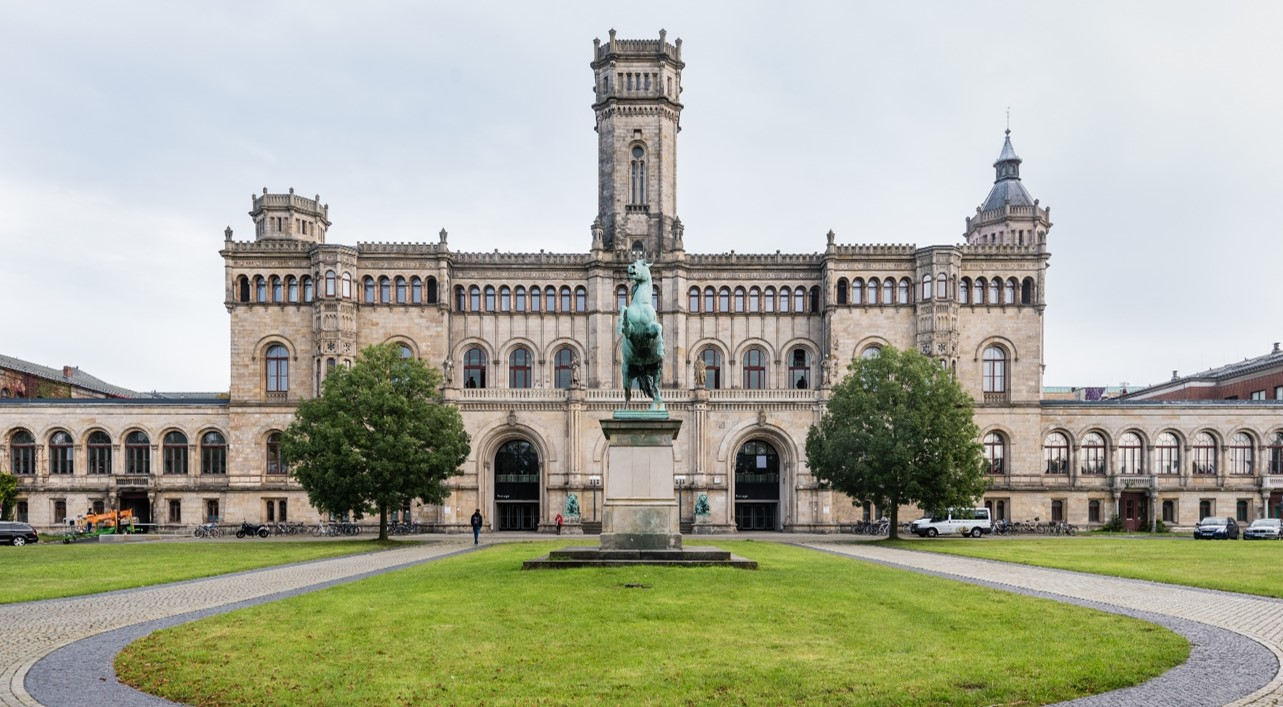
\includegraphics[width=0.65\textwidth]{figures/luh_default_presentation_title_image.jpg}}

% Title page: luhstyle
% \setbeamertemplate{title page}[luhstyle]
% % Add optional title image here
% \addtitlepageimage{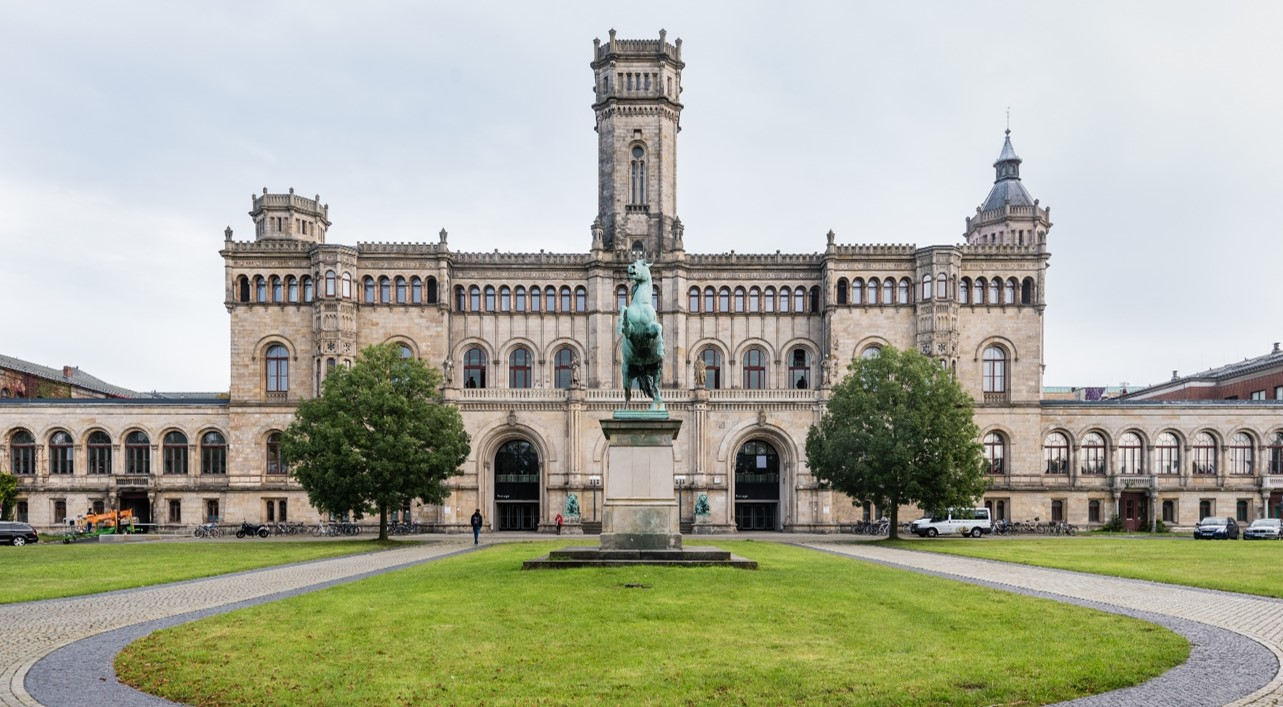
\includegraphics[width=0.75\textwidth]{figures/luh_default_presentation_title_image.jpg}}

\author[Abedjan \& Lindauer]{Ziawasch Abedjan \& Marius Lindauer\\[1em]
	
\includegraphics[height=\logoheight]{../latex_main/figures/luh_logo_rgb_0_80_155.pdf}\qquad
	
\includegraphics[height=\logoheight]{../latex_main/figures/DBIS_Kurzlogo.png}\qquad

\includegraphics[height=\logoheight]{../latex_main/figures/TNT_darkv4}\qquad

\includegraphics[height=\logoheight]{../latex_main/figures/L3S.jpg}	}
\date{Summer Term 2022; \hspace{0.5em} {
\includegraphics[height=1.5em]{../latex_main/figures/Cc-by-nc-sa_icon.svg.png}}; based on \href{https://ds100.org/fa21/}{[DS100]}
}


%%% Custom Packages
%----------------------------------------------------------------------
% Create dummy content
\usepackage{blindtext}

% Adds a frame with the current page layout. Just call \layout inside of a frame.
\usepackage{layout}


%%% Macros
%\renewcommand{\vec}[1]{\mathbf{#1}}
% \usepackage{bm}
%\let\vecb\bm

\title[Statistics]{DS: Bias and Variance}
\subtitle{Decomposition of Risk}

\graphicspath{ {./figure/} }
%\institute{}


\begin{document}
	
	\maketitle
	\begin{frame}{Model Risk}
	    For a new sample at $(x, Y)$:
	    \begin{itemize}
	        \item Expected mean squared error of prediction:
	        \begin{equation*}
	            \text{model risk} = \mathbb{E}\left[(Y-\widehat{Y}(x))^2\right]
	        \end{equation*}
	    \end{itemize}
	    The expectation is taken over all possible samples that we could have collected.
	    \begin{itemize}
	        \item Remember, each new sample would generate a different $\widehat{Y}(x)$
	        \item Also, for some fixed $x$, $Y$ can be different due to the random error $\epsilon$
	    \end{itemize}
	\end{frame}
	
	
	\begin{frame}[c]{Decomposition of Error and Risk}
	    The model risk can be decomposed into three pieces:
	    \begin{align*}
	        \mathbb{E}\left[(Y-\hat{Y}(x))^2\right] &= \mathbb{E}(\epsilon^2)\\
	        &+ (g(x) - \mathbb{E}(\hat{Y}(x)))^2\\
	        &+ \mathbb{E}\left[(\mathbb{E}(\hat{Y}(x))-\hat{Y}(x))^2\right]
	    \end{align*}
	    \begin{equation*}
	        \text{model risk} = \sigma^2 + (\text{model bias})^2 + \text{model variance}
	    \end{equation*}
	\end{frame}
	
	
	\begin{frame}[c]{Observation Variance (Noise)}
	    \begin{equation*}
	        \mathbb{V}ar(Y) = \mathbb{V}ar(g(x) + \epsilon) = \mathbb{V}ar(\epsilon) = \sigma^2
	    \end{equation*}
	    Some reasons:
	    \begin{itemize}
	        \item Measurement error
	        \item Missing information acting like noise
	    \end{itemize}
	    \bigskip
	    Some remedies:
	    \begin{itemize}
	        \item Could try to get more precise measurements.
	        \item Sometimes this is beyond the control of the data scientist.
	    \end{itemize}
	\end{frame}
	
	\begin{frame}[c]{Model Variance}
	    \begin{equation*}
	        \text{model variance} = \mathbb{V}ar(\hat{Y}(x)) = \mathbb{E}\left[(\hat{Y}(x) - \mathbb{E}(\hat{Y}(x)))^2\right]
	    \end{equation*}
	    Main reason:
	    \begin{itemize}
	        \item Overfitting: small differences in random samples lead to large differences in the fitted model
	    \end{itemize}
	    \bigskip
	    Some remedies:
	    \begin{itemize}
	        \item Reduce model complexity
	        \item Don’t fit the noise
	    \end{itemize}
	\end{frame}
	
	
	\begin{frame}[c]{Model Bias}
	    \begin{equation*}
	        \text{model bias} = \mathbb{E}(\hat{Y}(x)) - g(x)
	    \end{equation*}
	    Some reasons:
	    \begin{itemize}
	        \item Underfitting
	        \item Lack of domain knowledge
	    \end{itemize}
	    \bigskip
	    Remedies:
	    \begin{itemize}
	        \item Increase model complexity (but don’t overfit)
	        \item Consult domain experts to see which models make sense
	    \end{itemize}
	\end{frame}
	
	
	\begin{frame}[c]{A Constant Model}
	    So which model is better for a Bernoulli distribution with $p=.5$? Model A or Model B?\\
	    \bigskip
	    \textbf{Model A:} Select a random number between $0$ and $1$. This is your estimate of p.\\
        \textbf{Model B:}: Select $.75$ as your estimate of p.\\
        \bigskip
        We can calculate the model risks directly. Note that the observation variance is 0.
        \begin{columns}
            \begin{column}{.4\textwidth}
                  Model A:\\
                  \bigskip
                  Model Bias = .5 - .5 = 0\\
                  Model Variance = (1 - 0)$^2$ / 12 = 1/12\\
                  \bigskip
                  Risk = 0$^2$ + 1/12 = 1/12
            \end{column}
            
            
            \begin{column}{.4\textwidth}
                   Model B:\\
                  \bigskip
                  Model Bias = .75 - .5 = .25\\
                  Model Variance = 0\\

                  \bigskip
                  Risk = .25$^2$ + 0 = 1/16
 
            \end{column}
        \end{columns}

	\end{frame}
\end{document}